%------------------------------------------------------------
% Retro-25 calculators
%------------------------------------------------------------

\pdfminorversion=4   % fix Acrobat error
\documentclass{beamer}
\usepackage{graphicx}
\usepackage{tikz}    % for logo onlyh
\usepackage{xcolor}
\usepackage{hyperref}
\usepackage[absolute,overlay]{textpos}
\usepackage{makecell}
\usepackage{array}
\usepackage{makecell}
\usepackage{fancyvrb}

\definecolor{my-red}{RGB}{128,0,0}
\definecolor{my-green}{RGB}{0,96,0}
\definecolor{my-blue}{RGB}{0,0,128}
\definecolor{my-orange}{RGB}{160,83,0}
\definecolor{my-violet}{RGB}{142,0,209}
\definecolor{my-aqua}{RGB}{0,96,96}
\definecolor{my-olive}{RGB}{89,124,0}

\newcommand{\tred}[1]{\textcolor{my-red}{#1}}
\newcommand{\tgreen}[1]{\textcolor{my-green}{#1}}
\newcommand{\tblue}[1]{\textcolor{my-blue}{#1}}
\newcommand{\torange}[1]{\textcolor{my-orange}{#1}}
\newcommand{\tviolet}[1]{\textcolor{my-violet}{#1}}
\newcommand{\taqua}[1]{\textcolor{my-aqua}{#1}}
\newcommand{\tolive}[1]{\textcolor{my-olive}{#1}}

\renewcommand{\indent}{\hspace*{2em}}
\renewcommand{\arraystretch}{1.5}

\usepackage{hyperref}
\hypersetup{
    colorlinks=true,
    linkcolor=blue,
    filecolor=magenta,      
    urlcolor=cyan,
}
 
\urlstyle{same}

\begin{document}

% Add footer text
\addtobeamertemplate{footline}{
  \parbox{\linewidth}{\vspace*{-8pt}
    ~~~ Slide \insertframenumber/\inserttotalframenumber
    ~~~ 2020-10-10 ~~~
    E.~Hazen}
}

% Move footnotes above footline
\addtobeamertemplate{footnote}{}{\vspace{0.1in}}

% add BU + ATLAS logo
\addtobeamertemplate{frametitle}{}{%
\begin{tikzpicture}[remember picture,overlay]
\node[anchor=north east,yshift=2pt] at (current page.north east)
%{\includegraphics[height=0.8cm]{figs/BU_LOGO.png}};
{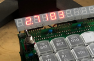
\includegraphics[height=0.8cm]{figs/retro.jpg}};
\end{tikzpicture}}

\title{The Retro-25 DIY Calculators}
\author
{
 \begin{center}
   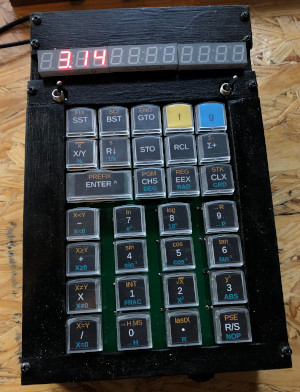
\includegraphics[height=3cm]{figs/led_front.jpg} 
   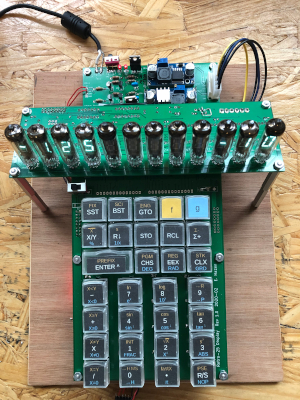
\includegraphics[height=3cm]{figs/vfd_over.jpg}
 \end{center}
E.~Hazen % \\
% representing myself only
}

\newcommand{\spage}[1]{
\begin{frame}
  \begin{tikzpicture}[remember picture, overlay]
  \node[anchor=north]at(current page.north){
     \includegraphics[width=0.95\paperwidth]{#1}
  };
  \end{tikzpicture}
\end{frame}
}
%% 
%% %---------- Title
\frame{\titlepage}

\begin{frame}
  \frametitle{Personal and Professional History...}
  \vskip -0.2in
  
  \begin{tabular}{p{0.7\textwidth}c}
  \scriptsize
  I've been fascinated by electronics since I was very young! & \\
    \scriptsize
    At age 13 (in 1973) I lived briefly in Leeds, England and worked
    at the Uni as an unpaid physics ``graduate assistant''.
    I encountered an HP-9100 and
    taught myself to program it.  I was immediately hooked! &
    \raisebox{-0.6\height}{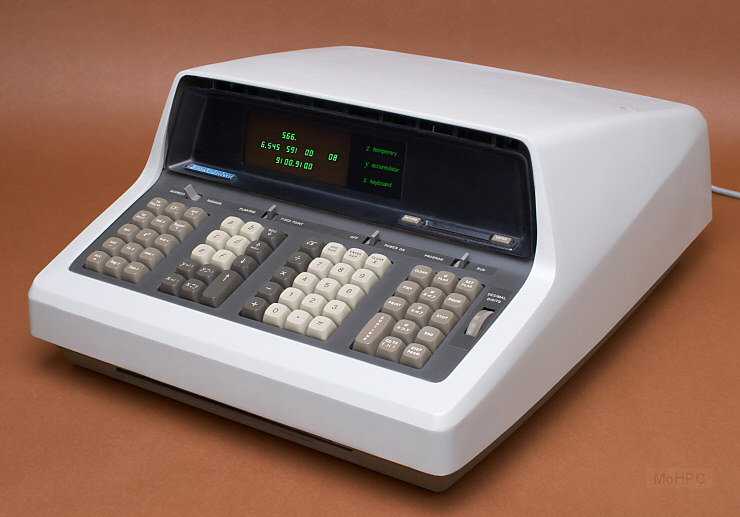
\includegraphics[width=1in]{figs/9100aqs.jpg}} \\
  \scriptsize
  In High School I made the acquaintance of an HP-2100 series
  computer running HP timeshare BASIC.  We played various games
  (some legit, like TREK73) and others (posting the administrator password
  on the chalkboard) not so legit.  &
    \raisebox{-0.8\height}{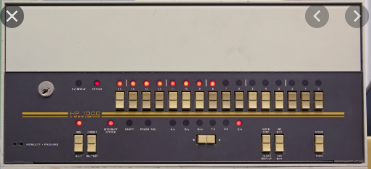
\includegraphics[width=1in]{figs/hp2100.jpg}} \\
    \scriptsize
    In 1975 my father bought an HP-25.
    I devoted myself to delivering the {\em Ann Arbor News}
    faithfully to about 60 subscribers, and eventually I could afford my
    own HP-25 at \$195.00 (about \pounds 663 today) &
    \raisebox{-0.6\height}{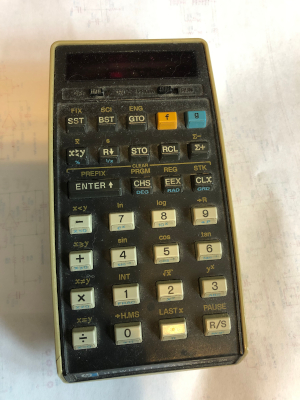
\includegraphics[width=0.5in]{figs/hp-25.jpg}} \\
    \scriptsize
    Unfortunately both HP-25 are now dead; mine fell in the fish tank with
    the piranhas while I was away and my roomies were scared to
    retrieve it!  My father's died when the batteries lost contact. &
    \raisebox{-0.6\height}{
\includegraphics[width=1in]{figs/piranha.jpg}} \\    

  \end{tabular}
\end{frame}

\begin{frame}
  \frametitle{...more history}
  \vskip -0.2in

  \begin{tabular}{p{0.7\textwidth}c}
  \scriptsize
  I studied computer science for a while at Michigan and
  became expert with the model 29 keypunch (I hated that thing!)
  I did learn a few other things (ALGOL and S/370 assembly) &
    \raisebox{-0.8\height}{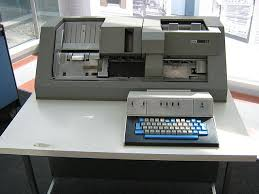
\includegraphics[width=0.7in]{figs/punch.jpg}} \\
  \scriptsize
  What really changed my life was working at Radio Shack.
  They introduced the TRS-80 and I immediately bought one
  (well, honestly, I put it on ``lay-a-way'' at my house!)
  I taught myself Z80 assembly language and wrote a simple multi-tasking
  kernel and FORTH system. &
    \raisebox{-0.8\height}{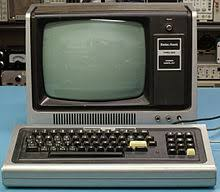
\includegraphics[width=0.7in]{figs/model1.jpg}} \\  
  \scriptsize
  I parlayed my Z80 skills into a job at ETC (theatre lighting).
  I designed their Idea$^{TM}$ and Vision$^{TM}$ lighting consoles, and wrote
  much of the low-level software in Z80 assembly (using my trusty
  TRS-80, now decked out with dual 8 inch floppies) as a dev system. &
    \raisebox{-0.8\height}{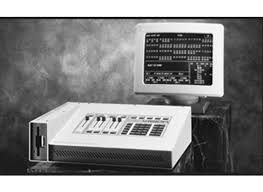
\includegraphics[width=1in]{figs/vision.jpg}} \\    
    \scriptsize
  Since then I've worked at Boston University building electronics
  mostly for the LHC at CERN.
  I've also become somewhat of an HP collector, acquiring a 10C,
    11C, 15C, 16C and 67.  The 10C and 15C were filched, the 11C and 16C
    I use almost daily.
&
  \raisebox{-0.8\height}{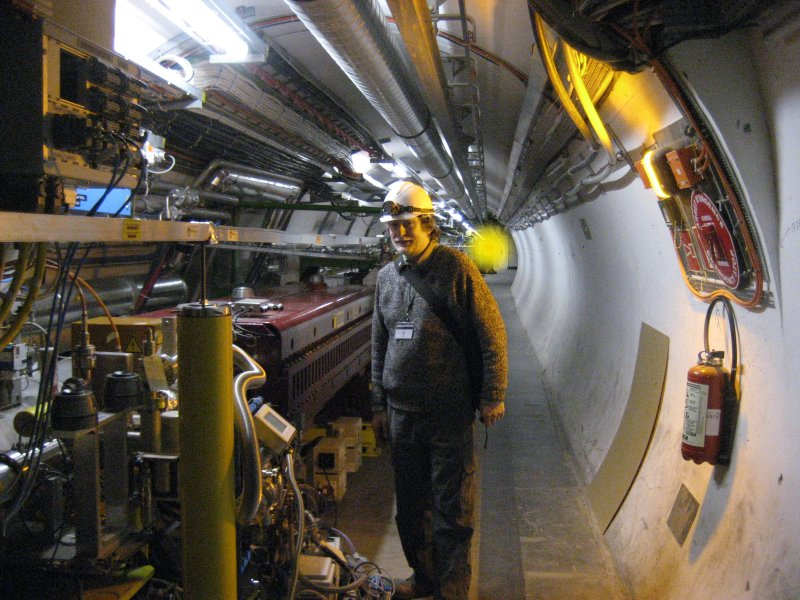
\includegraphics[width=1in]{figs/Tunnel.jpg}} \\    
  \end{tabular}
\end{frame}


\begin{frame}
  \frametitle{Why? Why? Why?}

  \begin{columns}
  \column{0.7\textwidth}
  \tblue{Why a DIY HP-25?}

    \begin{itemize}
    \scriptsize
    \item The HP-25 is my favorite calculator
    \item The display and keyboard are too small for middle-aged eyes
    \item I hate mouse- and touchscreen-based emulators \\ (no tactile feel)
    \item I have a bunch of time on my hands ({\em NOT!})
    \end{itemize}
    \vskip 0.1in
  
    \tblue{Why use a Z80?}
  
    \begin{itemize}
    \scriptsize
    \item I know them inside-out
    \item They were released about when the HP-25 came out
    \item I like designing and assembling good old thru-hole DIP boards
    \end{itemize}
    \vskip 0.1in
  
    \tblue{Why the HECK VFD displays?}
    \begin{itemize}
    \scriptsize
    \item Because they are {\em cool!} \\
     (and nixies are a lot of trouble)
    \end{itemize}

  \column{0.3\textwidth}

    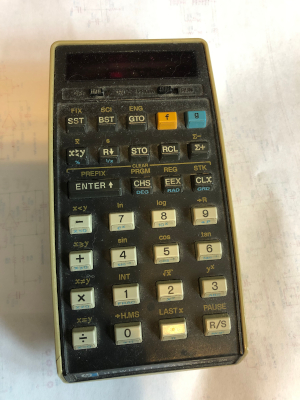
\includegraphics[width=0.7in]{figs/hp-25.jpg}
    \vskip 0.1in
    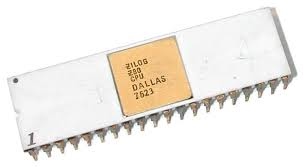
\includegraphics[width=1in]{figs/z80.jpg}
    \vskip 0.3in
    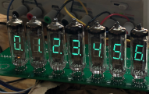
\includegraphics[width=1in]{figs/vfd.png}

  \end{columns}
\end{frame}

\begin{frame}
  \frametitle{Specification}

  Well, this is a hobby project so no spec needed, but I had goals:
    \begin{itemize}
    \item Big, clicky buttons; display I can read without glasses
    \item Simple hardware I could solder easily
    \item Cross-development from my Linux machine
    \end{itemize}

\end{frame}

\begin{frame}[shrink=5]
  \frametitle{Parts! Parts! Parts!}

  \vskip -0.15in
  \tgreen{I always start with the parts.}

    \scriptsize
  \begin{tabular}{p{0.7\textwidth}c}
    CPU: The Z80 is a no-brainer (initially Z80A, 4MHz) & 
     \raisebox{-0.5\height}{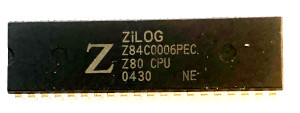
\includegraphics[width=1in]{figs/z80_black.jpg}} \\
     \hline
     \makecell[l]{Memory: first considered UV EPROM (nah!) \\
    AT28C256-15 EEPROM and 62256LP-70 RAM (both 32k, DIP-28)} & 
     \raisebox{-0.5\height}{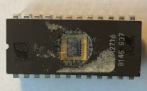
\includegraphics[width=0.7in]{figs/uveprom.jpg}} \\
     \hline
     \makecell[l]{Display: \\ 
                        V1: 10mm red 10mm red common anode 7-segment \\
                        V2: IV-6 green vacuum fluorescent display tubes}
     &
     \raisebox{-0.5\height}{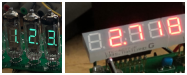
\includegraphics[width=1.3in]{figs/displays.png}} \\
     \hline
    Driver:  ICM7218A MUX driver.  I used these for
    theatre lighting consoles back in the day and they work well. & 
     \raisebox{-0.5\height}{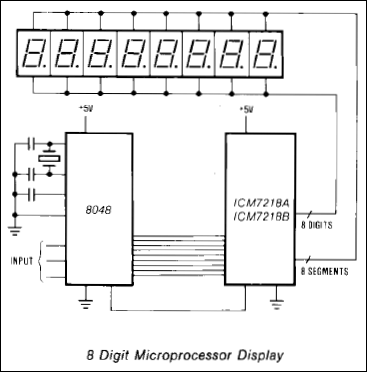
\includegraphics[width=0.7in]{figs/icm7218_ckt.png}} \\
     \hline
    Switches:  Cherry MX1A mechanical.  These are my favorites! &
     \raisebox{-0.3\height}{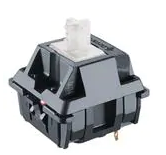
\includegraphics[width=0.7in]{figs/cherry.jpg}} \\
     \hline
  \end{tabular}

  \vskip 0.15in
  Otherwise, I have drawers full of 74LS and 74S series TTL at work
  because we can't bear to throw anything....

\end{frame}


\begin{frame}
  \frametitle{Boards!}

  \scriptsize
  How many boards?  Started with a ``toy'' layout in ExpressPCB to
  see how everything fit.  Looked like about 120x170mm.  So, I fired
  up KiCAD and made a schematic and did a layout.

  \vskip 0.15in

  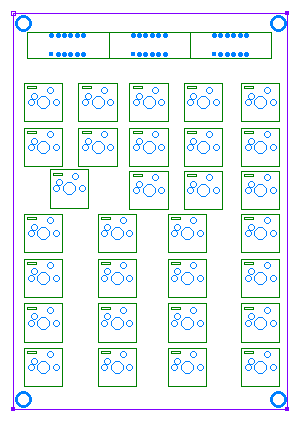
\includegraphics[width=1.5in]{figs/sample_epcb.png}

\end{frame}


\begin{frame}
  \frametitle{Schematics (KB, Display)}  

  \vskip -0.2in
  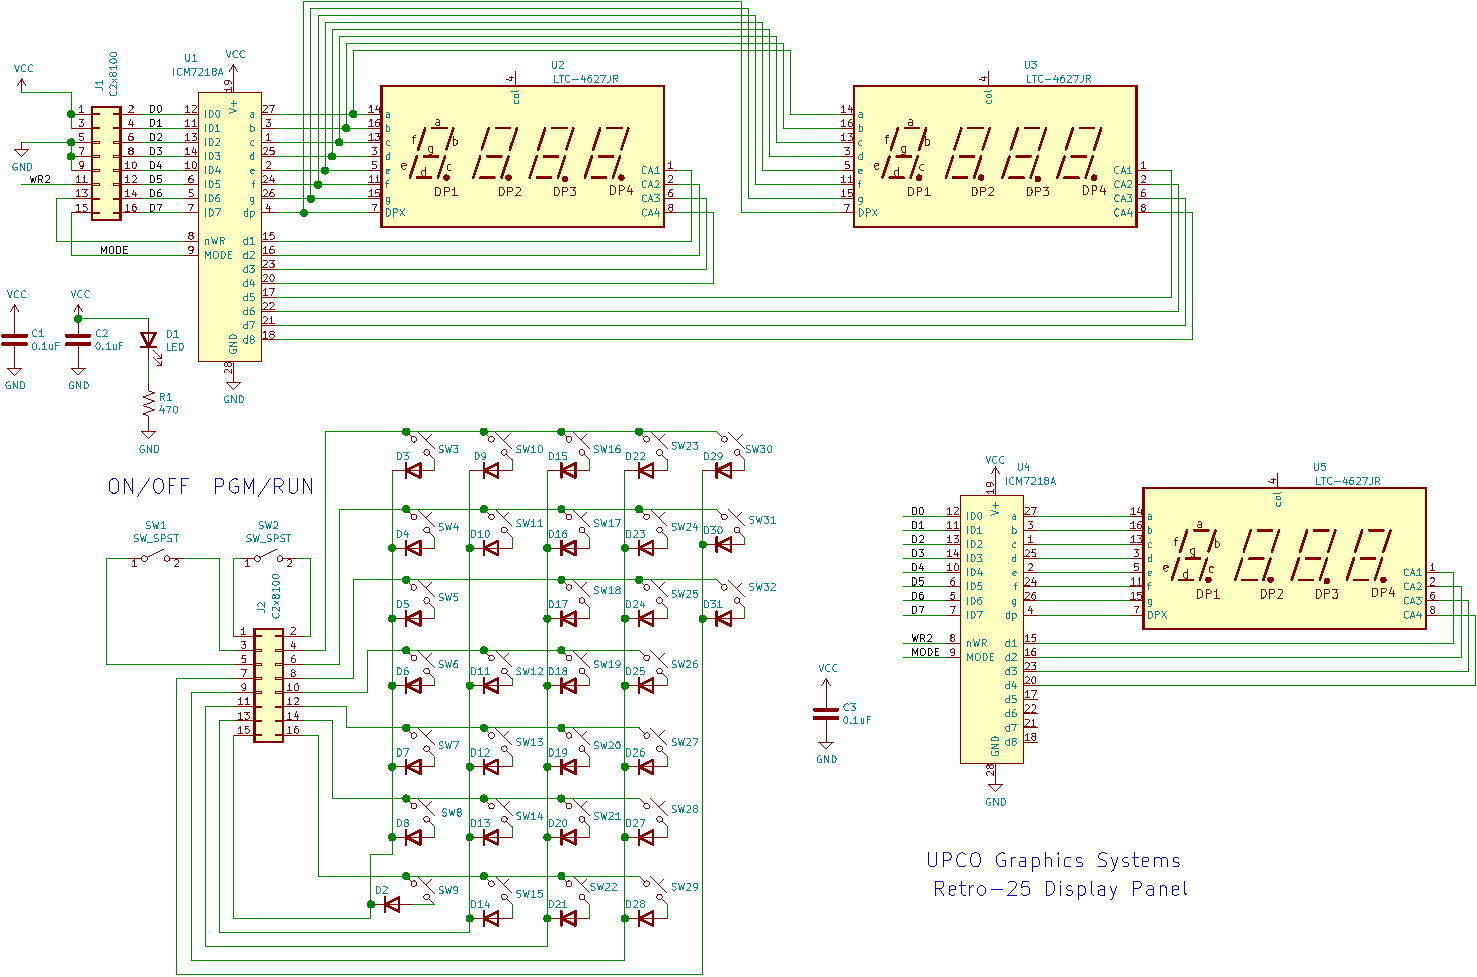
\includegraphics[width=\textwidth]{figs/led-display-crop.pdf}

  \scriptsize
  \begin{columns}
  \column{0.5\textwidth}
  \tblue{Keyboard is standard matrix}
  \column{0.5\textwidth}
  \tred{Display handled by two ICM7218A.  \\ Almost no additional parts}
  \end{columns}
\end{frame}

\begin{frame}
  \frametitle{PCB (KB, Display)}

  \vskip -0.2in
  \scriptsize
  \begin{columns}
  \column{0.5\textwidth}
    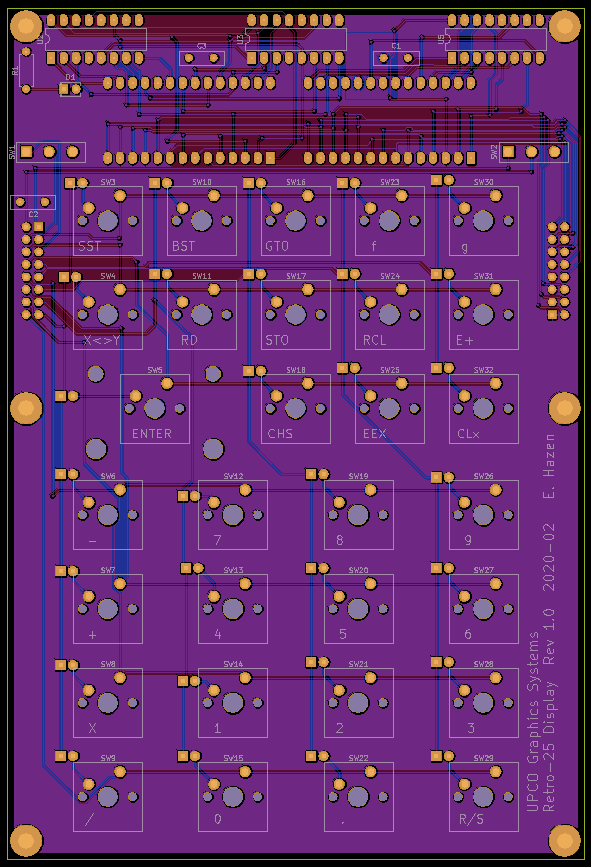
\includegraphics[width=\textwidth]{figs/led-gerbers.png}        
  \column{0.5\textwidth}
  
    Placement and routing pretty simple. \\
    Two header connectors, one for KB and one for LEDs
    \vskip 0.2in
    \tviolet{Top Cu area to GND} \\
    \tred{Bottom Cu area to VCC} \\
    \vskip 0.2in
    Design rules based on what JLCPCB could do easily: \\
    \tgreen{
    ~~ 6 mil line/space (0.15 mm)\\
    ~~ 20 mil via with 10 mil hole \\ ~~~~(0.5mm / 0.25mm)} \\
    \vskip 0.2in
    \tblue{Switches and LEDs take up most of front} \\
    \vskip 0.2in
    \tred{Diodes and LED drivers on back} \\
\end{columns}
\end{frame}

\begin{frame}
  \frametitle{Schematics (CPU)}

  \vskip -0.2in
  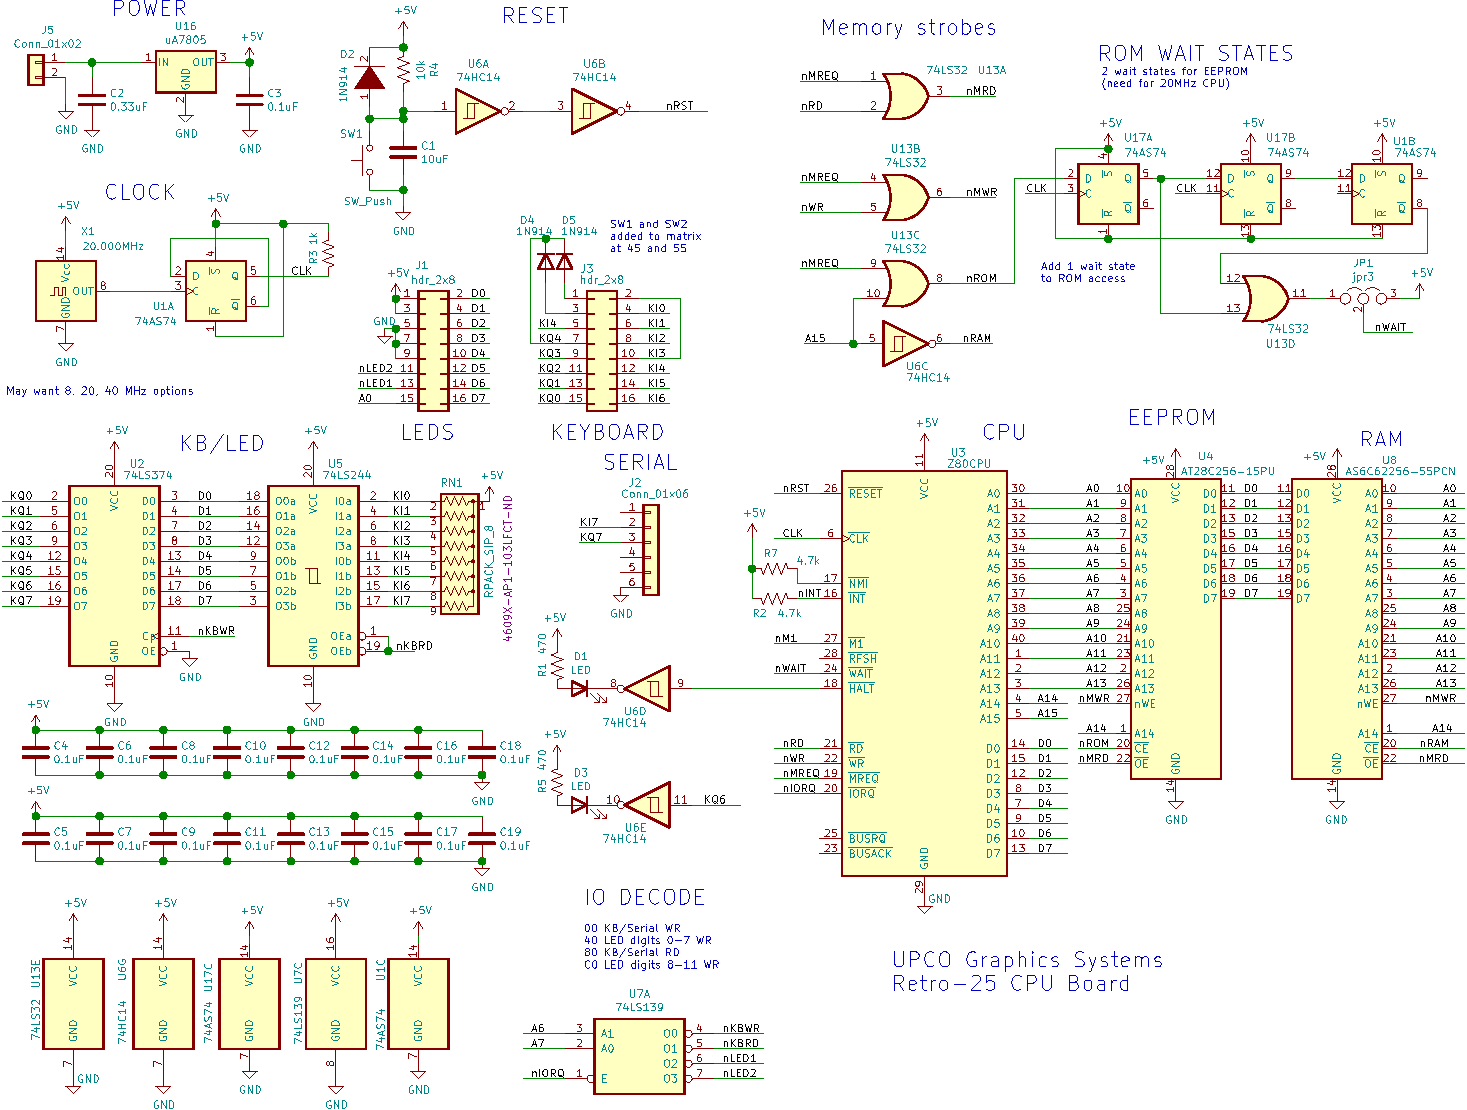
\includegraphics[width=\textwidth]{figs/cpu-sch-crop.pdf}

\end{frame}



\begin{frame}
  \frametitle{PCB (CPU)}

  \vskip -0.2in
  \scriptsize
  \begin{columns}
  \column{0.5\textwidth}
    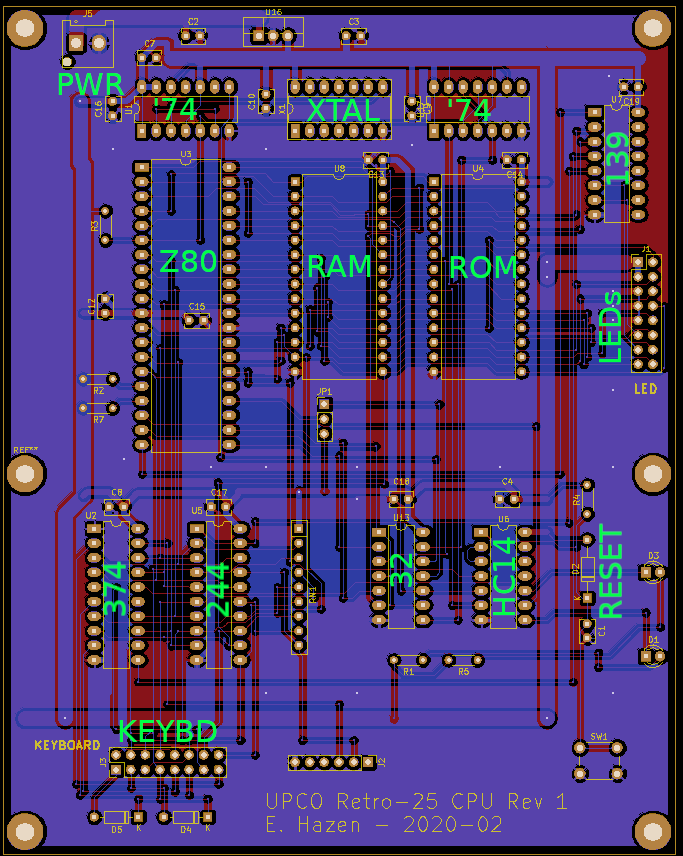
\includegraphics[width=\textwidth]{figs/cpu-board.png}
  \column{0.5\textwidth}
  
    Placement and routing pretty simple. \\
    Two header connectors, one for KB and one for LEDs \\
    All components on the top.
    \vskip 0.2in
    \tviolet{Top and bottom Cu areas to GND} \\
    \vskip 0.2in
    \tblue CPU, RAM, EEPROM in top row
    \vskip 0.2in
\end{columns}
\end{frame}


\begin{frame}
  \frametitle{Bringing it Up! (hardware)}
  \begin{columns}
  \column{0.5\textwidth}
    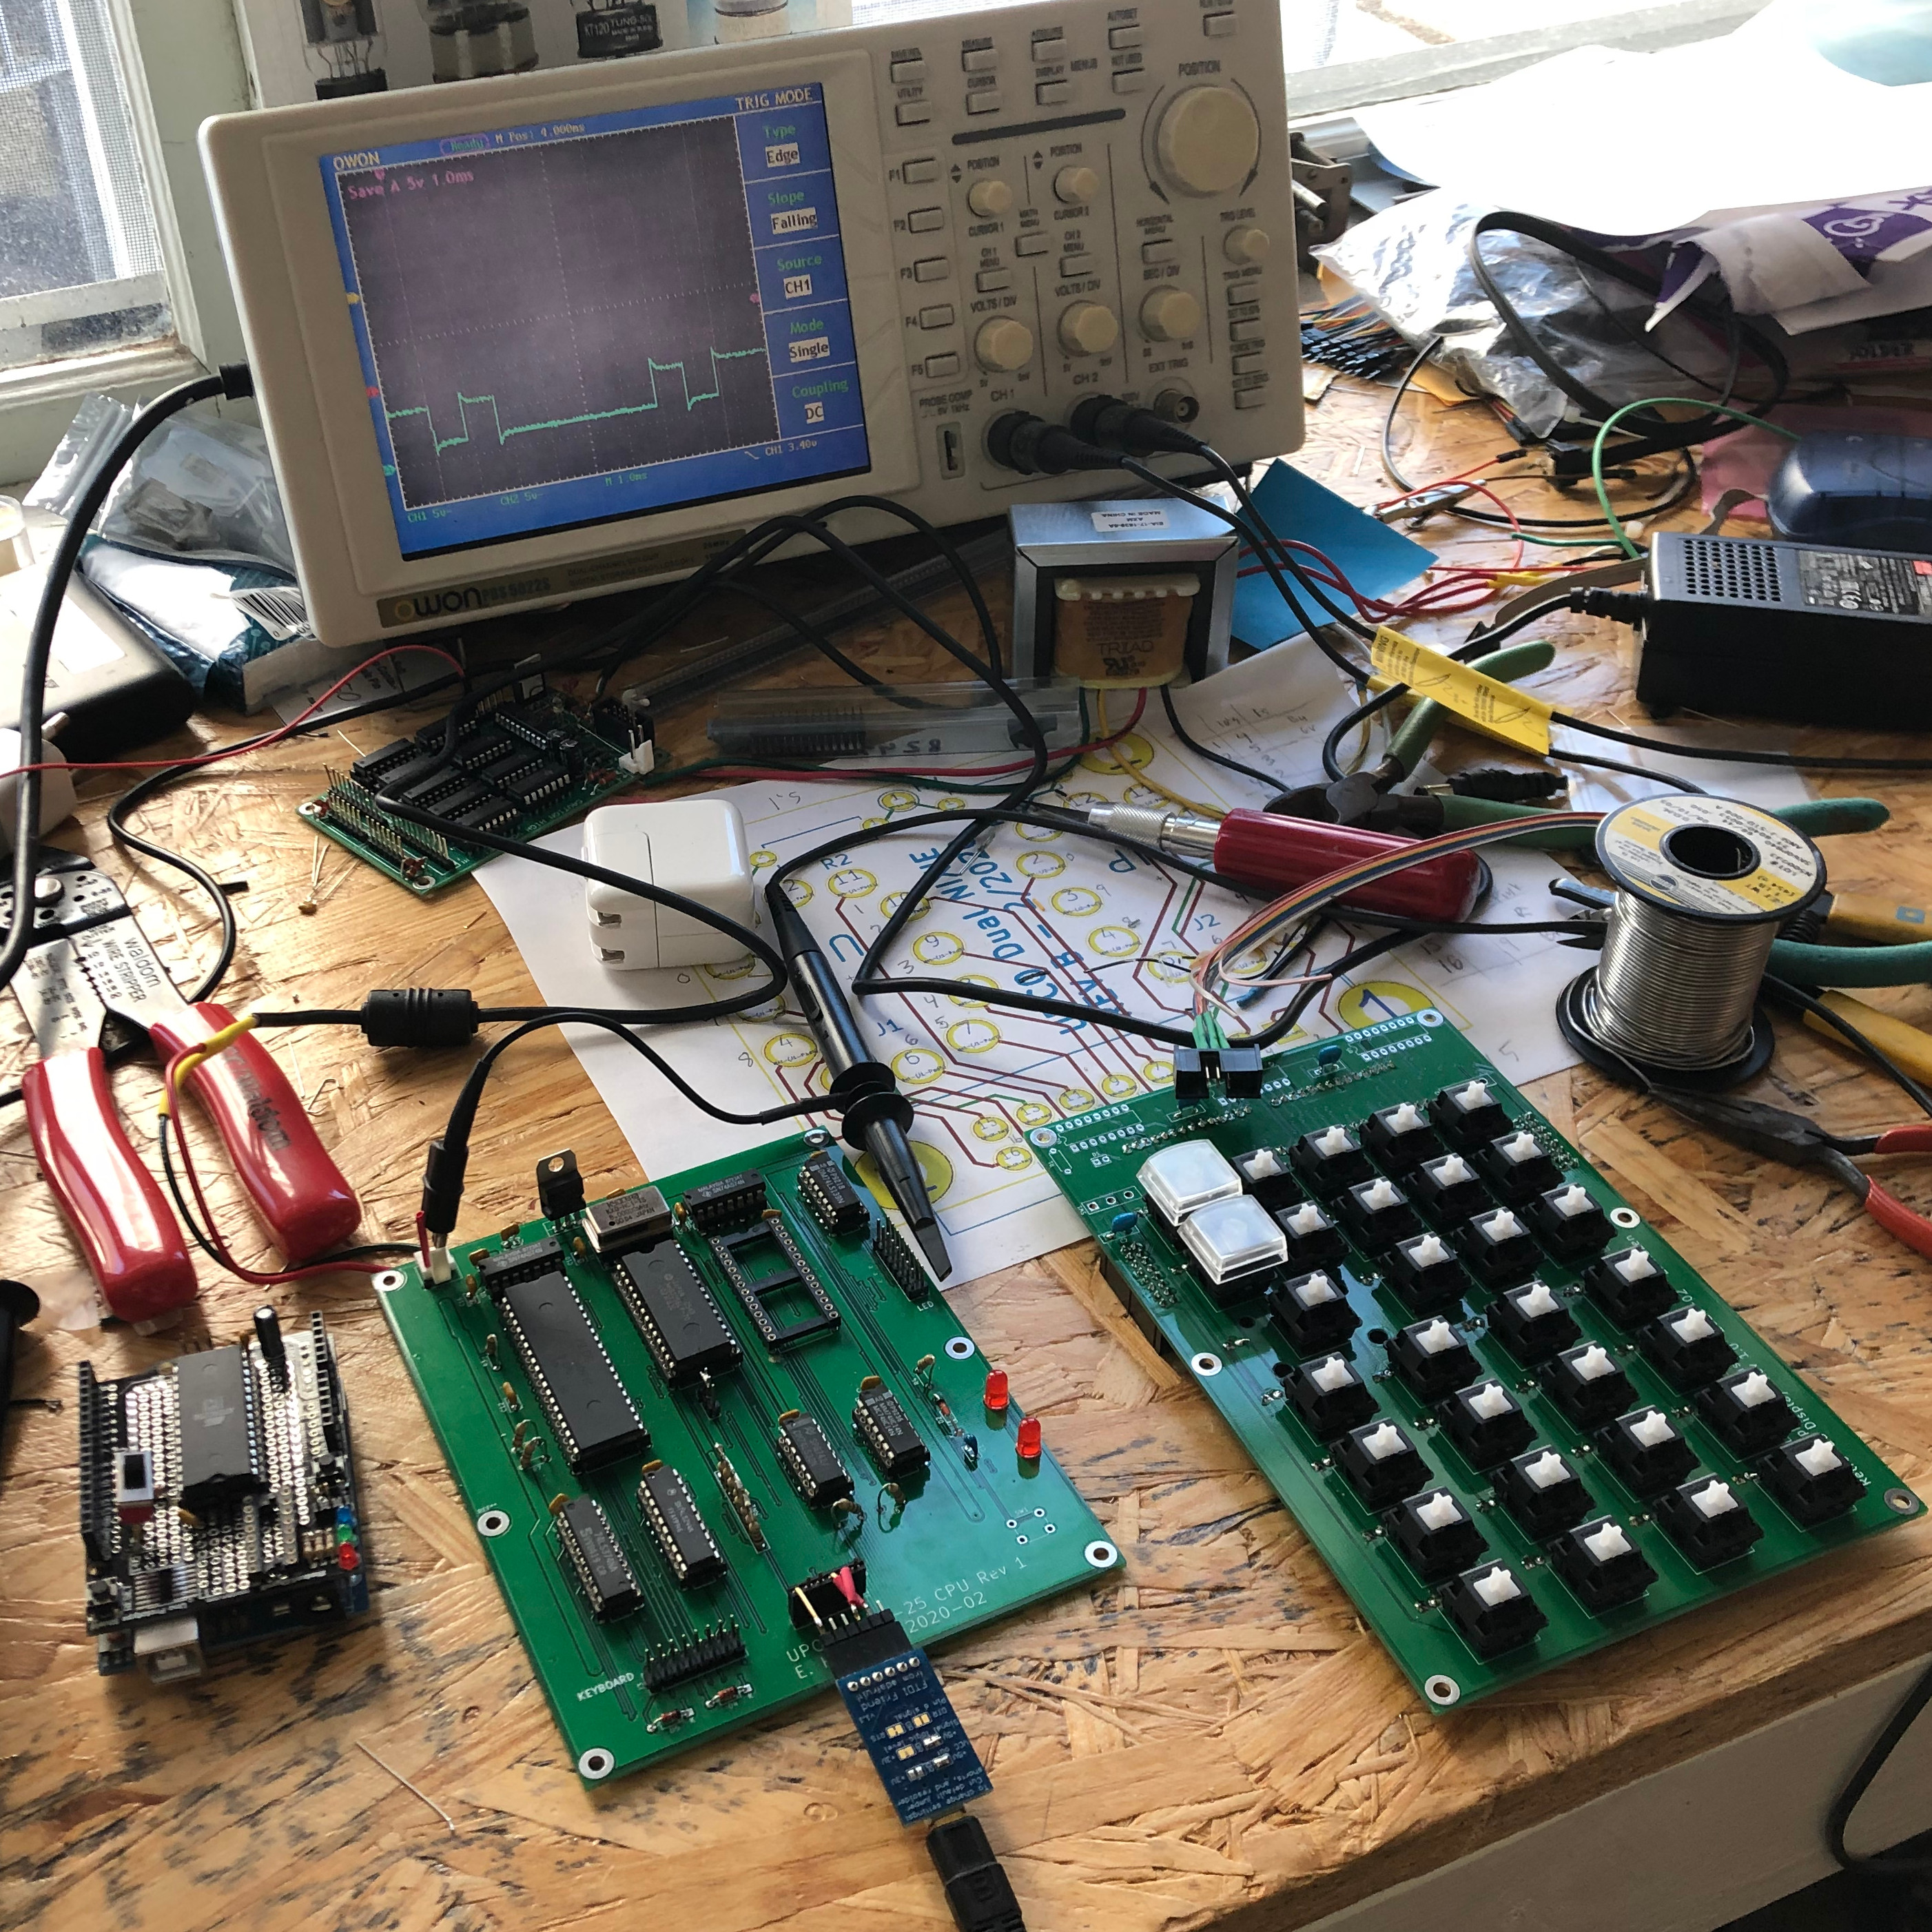
\includegraphics[width=\textwidth]{figs/bench.jpg}
  \column{0.5\textwidth}
    \tgreen{The boards and parts are here!}
    \begin{itemize}
    \scriptsize
    \item Easy soldering (all thru-hole) \\
      But then what?  Software?
    \item Brief diversion to make a junk-box EEPROM programmer
    \item First program:  delay, then HLT \\
       i.e. {\tt 2B 7C B5 20 FB 76} \\
       (glad I put a HALT LED on the board!)
    \item Then a struggle with bit-bang serial \\
       (next time use a UART!)
    \item Then write a debug monitor... ``umon2''.
    \end{itemize}
    \tred{Two months later...}
\end{columns}
\end{frame}

\begin{frame}
  \frametitle{Bringing it Up!  (software)}
  \begin{columns}
  \column{0.4\textwidth}
    \scriptsize
    
\includegraphics[width=\textwidth]{figs/nonpareil.png} \\
    \url{http://nonpareil.brouhaha.com} \\
    \vskip 0.1in
    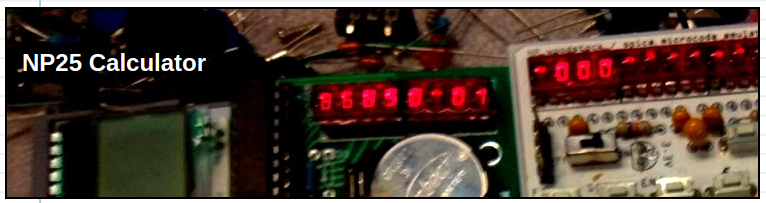
\includegraphics[width=\textwidth]{figs/np25.png} \\
    \url{http://simpleavr.github.io/NP25/} \\
    \vskip 0.1in
    
\includegraphics[width=0.3\textwidth]{figs/z88dk.png} \\
    \url{https://github.com/z88dk/z88dk}
    \vskip 0.1in
    
\includegraphics[width=\textwidth]{figs/z80-sim.png} \\
    \url{https://www.autometer.de/unix4fun/z80pack/}
  \column{0.6\textwidth}
    \tgreen{Download and study...}
      \begin{itemize}
      \scriptsize
      \item Nonpareil by Eric Smith \\
        Very complete, but quite complex as it supports
        many models
      \item NP25 ``Nonpareil Physical'' by Chris Chung \\
        Woodstock-only emulator for MSP430 \\
        Much more promising
      \end{itemize}
    \scriptsize

    \vskip 0.1in
    \tblue{In the end I took some of both, and got an HP-25 only
      simulation running in plain C under linux, using a tty
      for input and output.} \\

    \vskip 0.1in
    \tviolet{Then, I built it using {\tt sdcc} in Z88DK and tested
      it under the {\tt z80pack} simulator.}
%    \tgreen{
  \end{columns}
\end{frame}

\begin{frame}[fragile]
  \frametitle{Bringing it Up!  (hardware+software)}

  \begin{columns}
  \column{0.75\textwidth}
  \scriptsize
  \vskip -0.2in
  \tgreen{Lots of loose ends...} \\
  \vskip 0.1in
  \tblue{First, write a serial boot loader} \\
  \vskip 0.1in
  \tblue{Then write a C program to send hex files} \\
  \vskip 0.1in
  \tblue{Then, work on the monitor...} \\
\begin{Verbatim}[fontsize=\tiny]
  d <addr> <count>         dump memory
  e <addr> <dd> <dd>...    edit up to 16 bytes in memory
  o <port> <val>           output <val> to <port>
  z <val>                  set port zero value bits 0-6
  i <port>                 input from <port> and display
  g <addr>                 goto addr
  b <addr>                 set breakpoint (currently 3-byte call)
  a <val1> <val2>          hex Arithmetic
  c                        continue from breakpoint
  c <addr>                 continue, set new breakpoint
  m <start> <end> <size>   memory region compare
  p <start> <end> <size>   memory region copy
  l                        binary load from serial
  r                        repeat last command
  k                        scan HP keyboard
  f <addr>                 dump HP registers from <addr> (A)
  7 <addr>                 update 7-segment display from <addr>
  V <addr>                 update VFD display from <addr>
\end{Verbatim}
  \tred{I eventually needed all of those commands...} \\
  \vskip 0.1in
  \tgreen{Finally, start to load and debug the calculator} \\
  \tgreen{Before long, it works!!}
  \column{0.25\textwidth}

  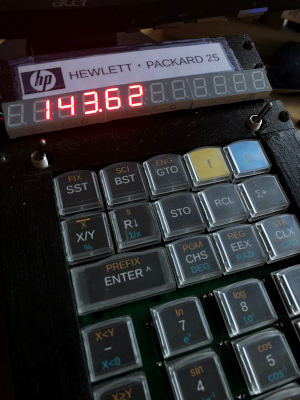
\includegraphics[width=\textwidth]{figs/led-close.jpg}

  \end{columns}
\end{frame}

\begin{frame}
  \frametitle{Wrapping it Up}
  \framesubtitle{}
  \begin{tabular}{cp{0.5\textwidth}{c}}
    \raisebox{-0.6\height}
      {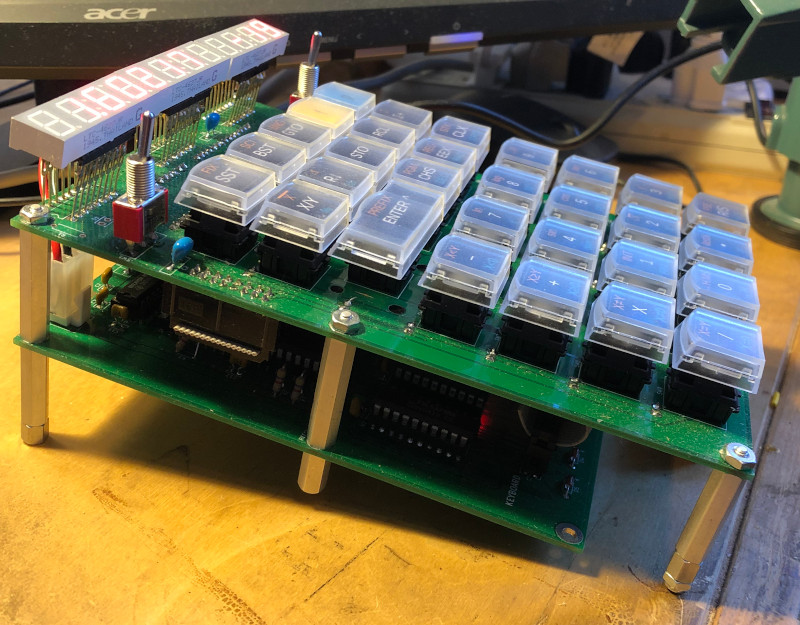
\includegraphics[width=0.3\textwidth]{figs/side_view.jpg}} &
    \scriptsize
    Stack the boards, add ``on/off'' and ``prgm/run'' switches,
    Make a simple wood box, it's done!
    \\
    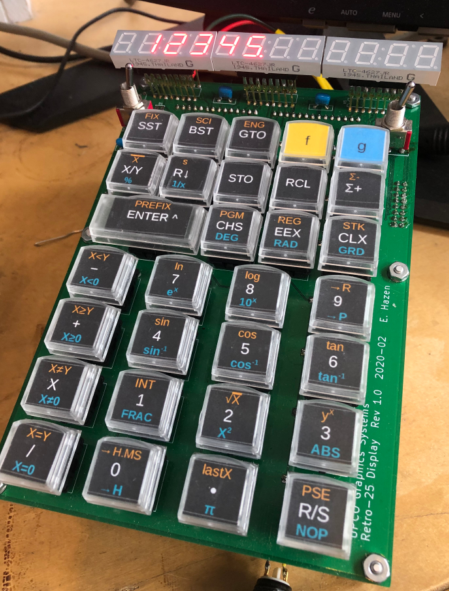
\includegraphics[width=0.3\textwidth]{figs/display-board.jpg} &
    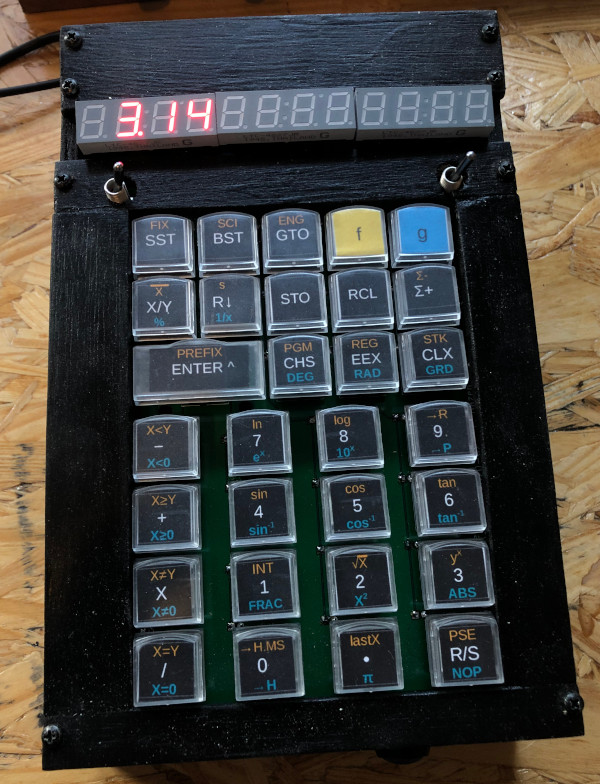
\includegraphics[width=0.3\textwidth]{figs/box_view.jpg} \\
  \end{tabular}
\end{frame}

\begin{frame}
  \frametitle{What Next?}
  \framesubtitle{S/N 2, of course!}

  \scriptsize

  \begin{columns}
  \column{0.3\textwidth}
    \tgreen{LEDs are boring! \\ Nixies are troublesome!} \\
    \vskip 0.1in
    \tred{Let's try VFDs... never used them before} \\
    \vskip 0.5in
    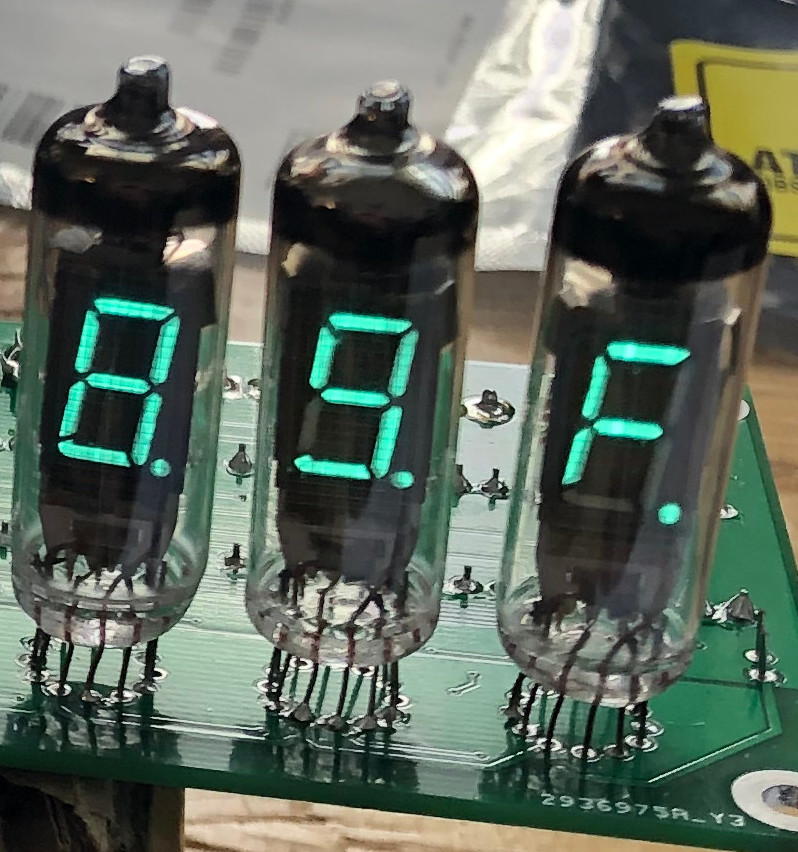
\includegraphics[width=0.7\textwidth]{figs/vfd-closeup.jpg}
  \column{0.75\textwidth}
    \tblue{My Russian isn't so good, but Google Translate to the rescue...} \\
    \vskip 0.2in
    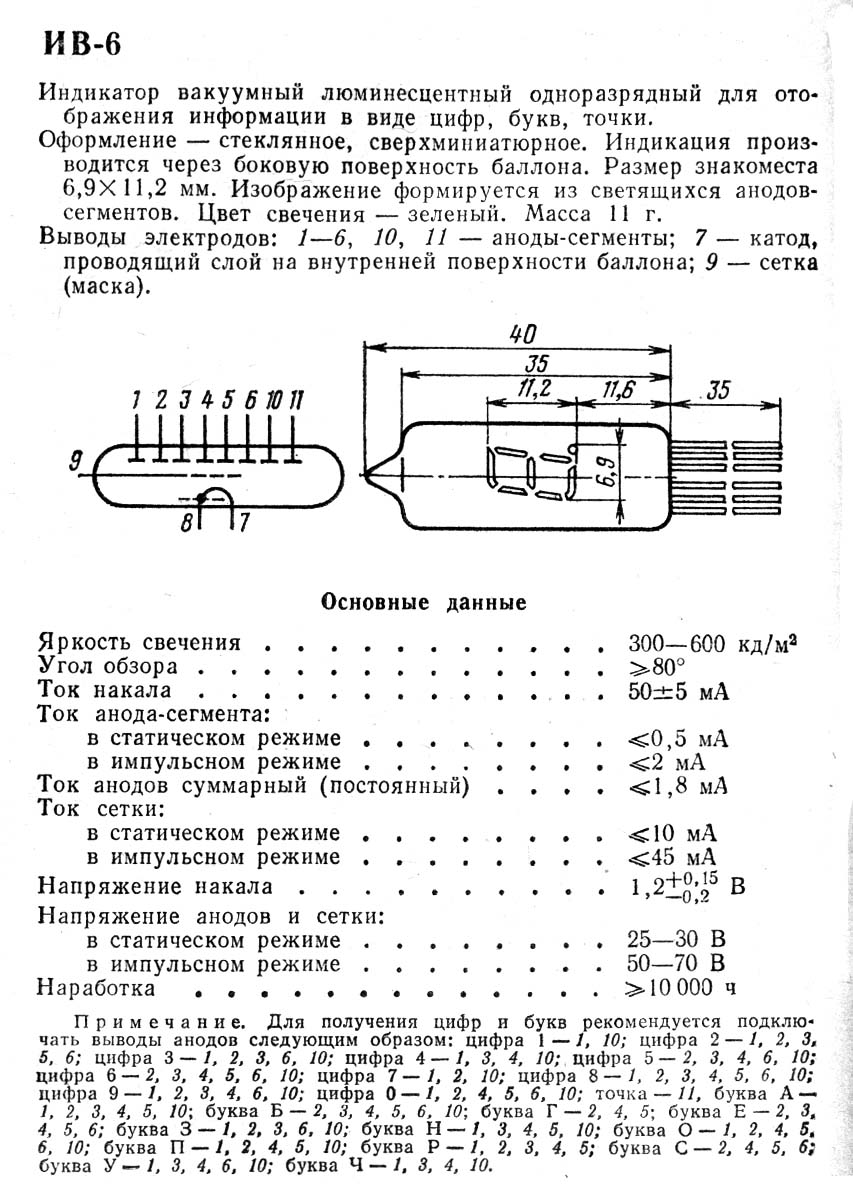
\includegraphics[width=0.45\textwidth]{figs/iv-6-datasheet.jpg}
    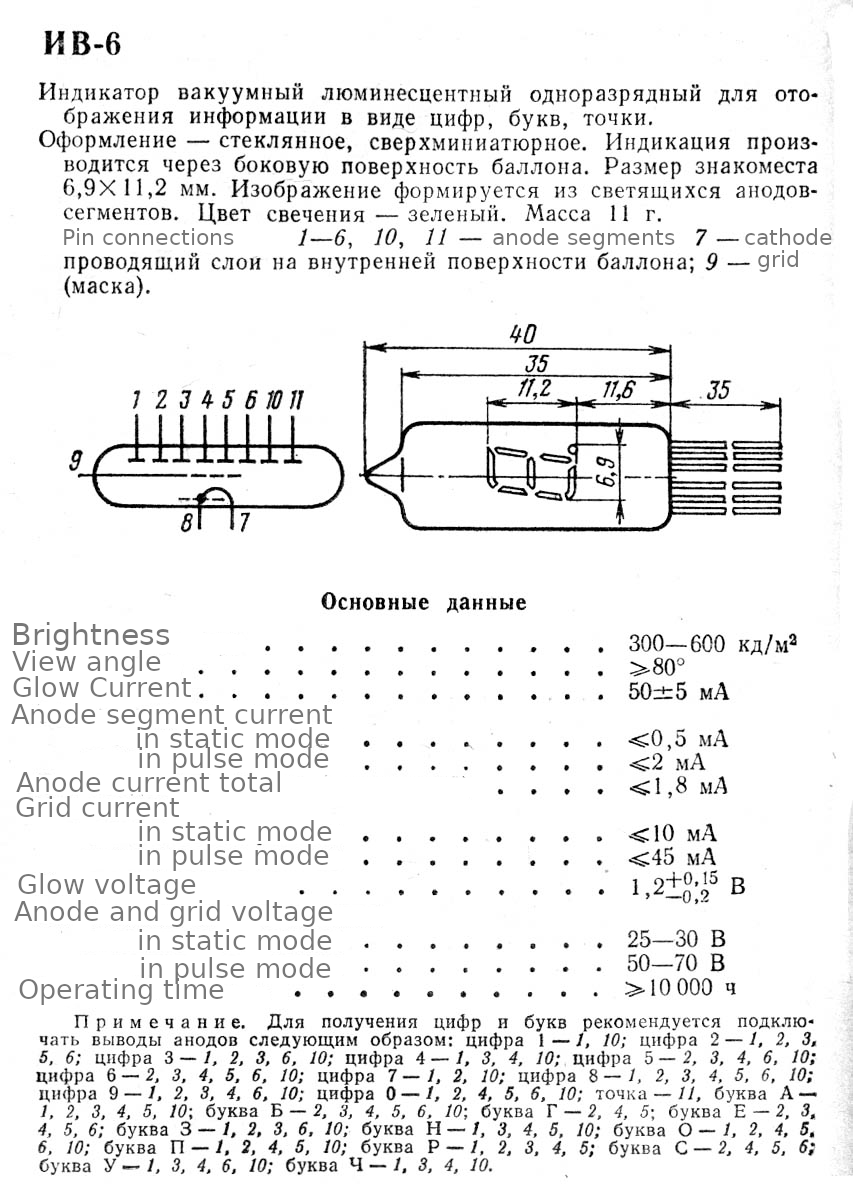
\includegraphics[width=0.45\textwidth]{figs/iv-6-datasheet-translated.png}
  \end{columns}
\end{frame}

\begin{frame}
  \frametitle{VFD Display Board}
  \framesubtitle{Schematic}
  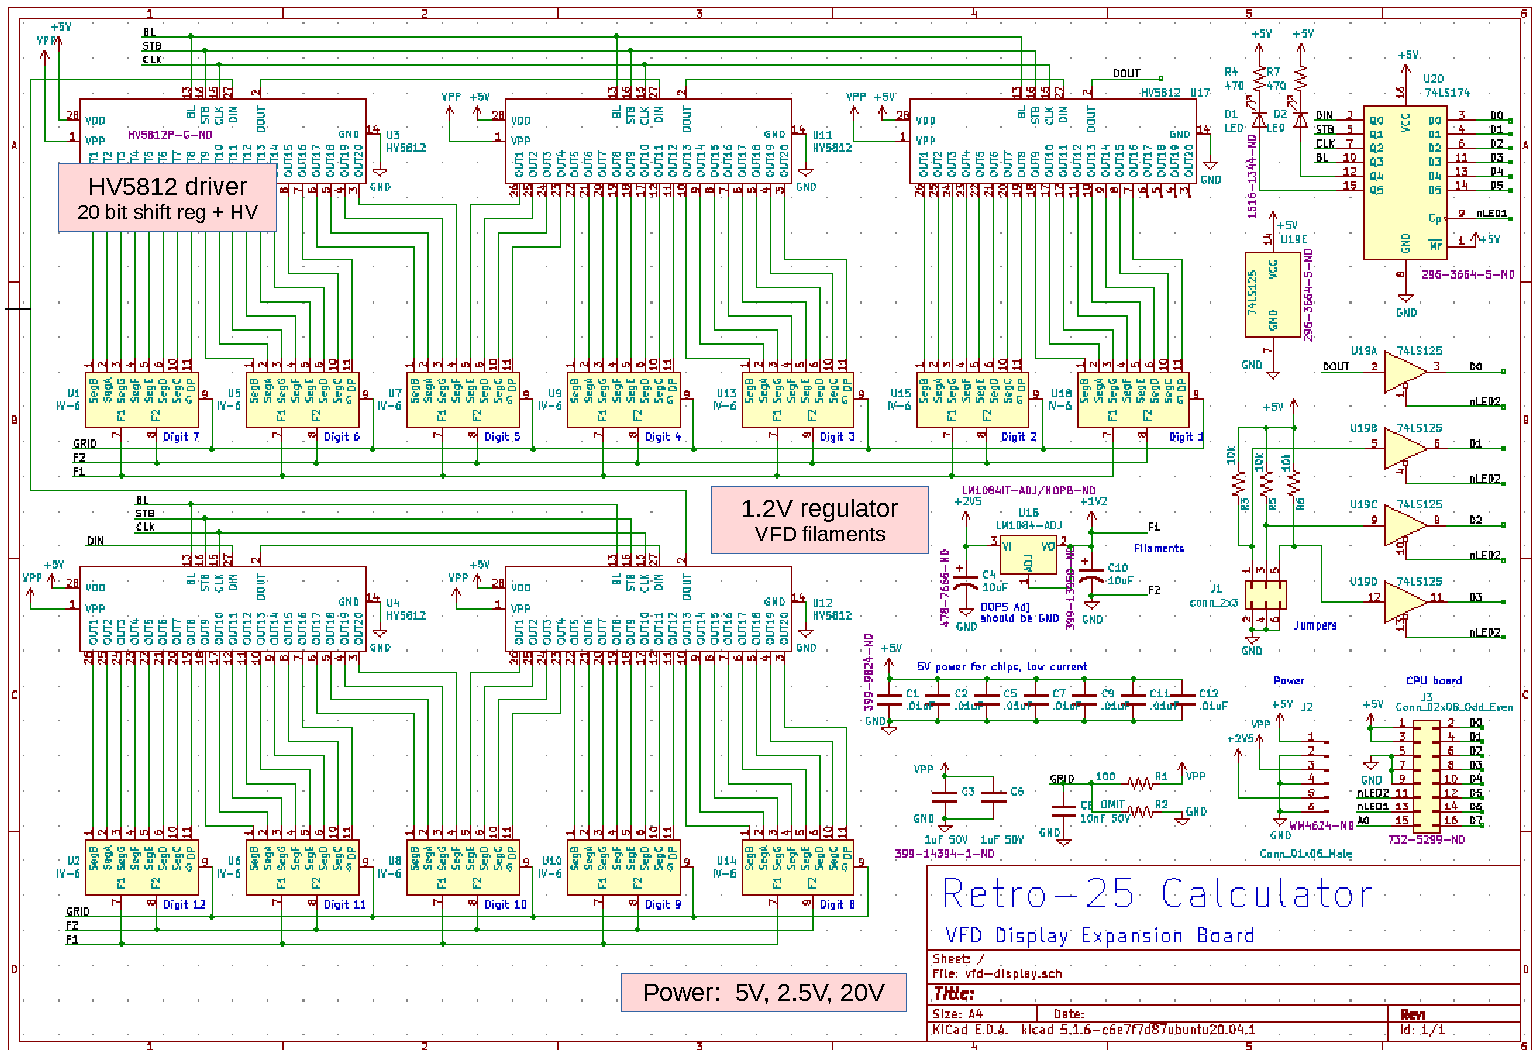
\includegraphics[width=\textwidth]{figs/vfd-schem-ann.pdf}
\end{frame}

\begin{frame}
  \frametitle{VFD Display Board}
  \framesubtitle{PCB Design}
  \begin{columns}
  \column{0.7\textwidth}
    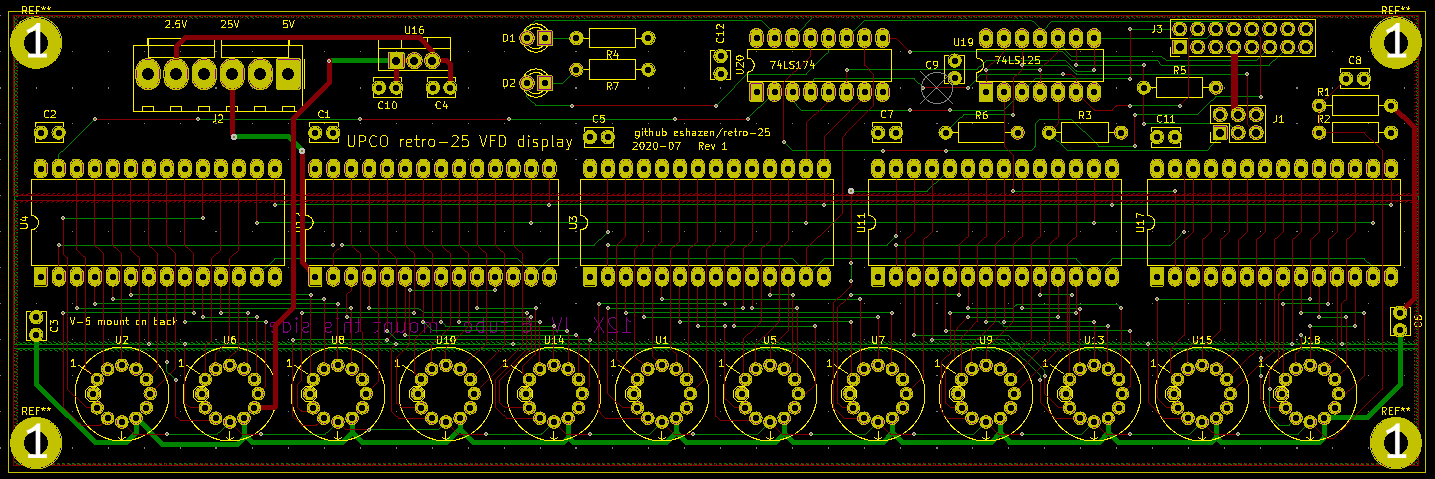
\includegraphics[width=\textwidth]{figs/vfd-layout.jpg} \\ 
    \vskip 0.2in
    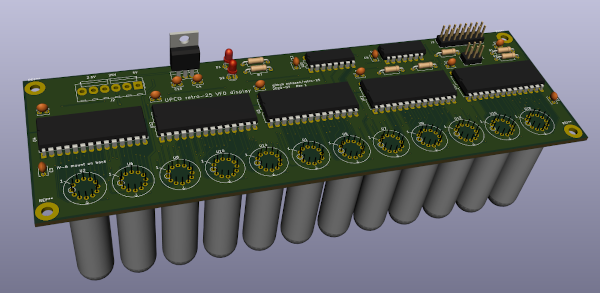
\includegraphics[width=\textwidth]{figs/render_board.png}
  \column{0.4\textwidth}
    \begin{itemize}
    \scriptsize
    \item 12 display tubes
    \item 5 HV5812 driver chips
    \item 2 TTL chips
    \item 1.2V @ ~1A for filaments
    \item Power connector (5V, 2.5V, 20V)
    \item Ribbon cable compatible with LED board
    \item Two layer, pretty simple layout
    \item Fun with 3D modeling!
    \end{itemize}
  \end{columns}
\end{frame}

\begin{frame}
  \frametitle{VFD Power Supply}
  \vskip -0.2in
  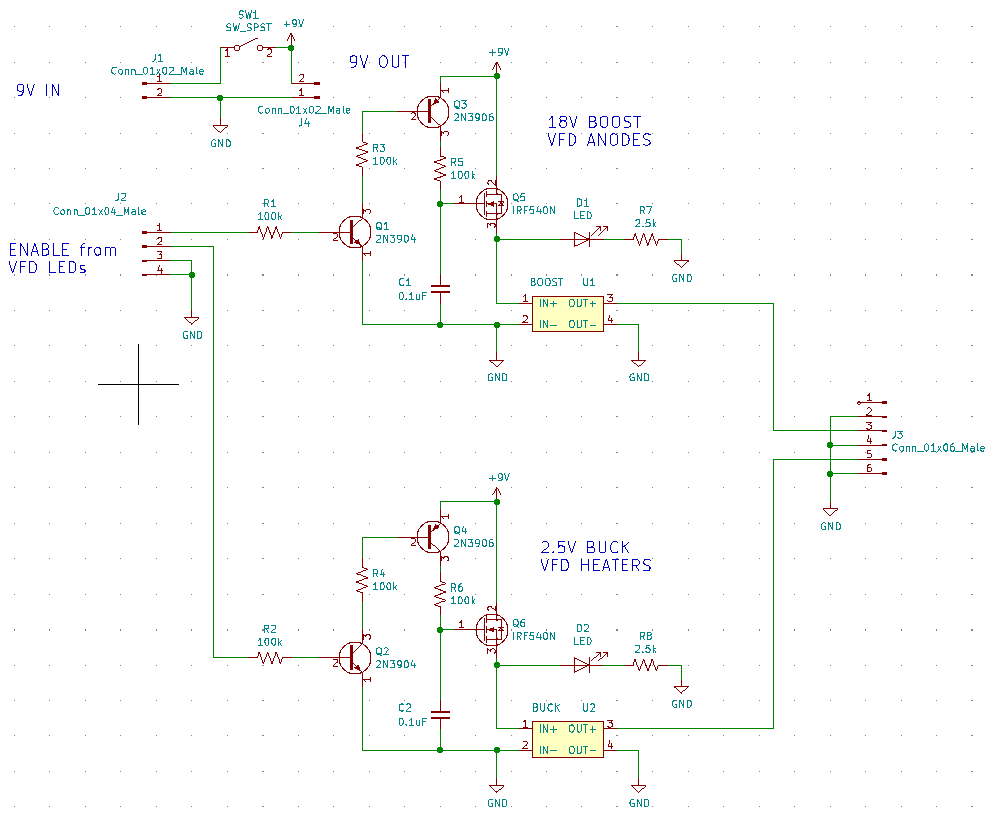
\includegraphics[width=0.7\textwidth]{figs/vfd-ps-schem.png} \\
  \scriptsize
  \tblue{VFD require noticeable power:} \\
  \tred{1.2V @ 0.6A (filaments), 20V @ 0.6A (plates)} \\
  \tgreen{So, another board!}
\end{frame}

\begin{frame}
  \frametitle{VFD Power Supply}

  \begin{columns}
  \column{0.5\textwidth}
  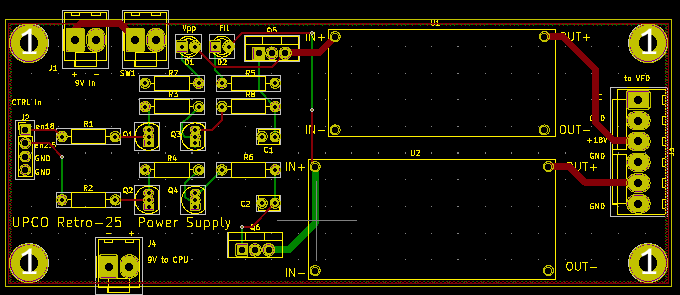
\includegraphics[width=\textwidth]{figs/vfd-ps-layout.png} \\
  \vskip 0.2in
  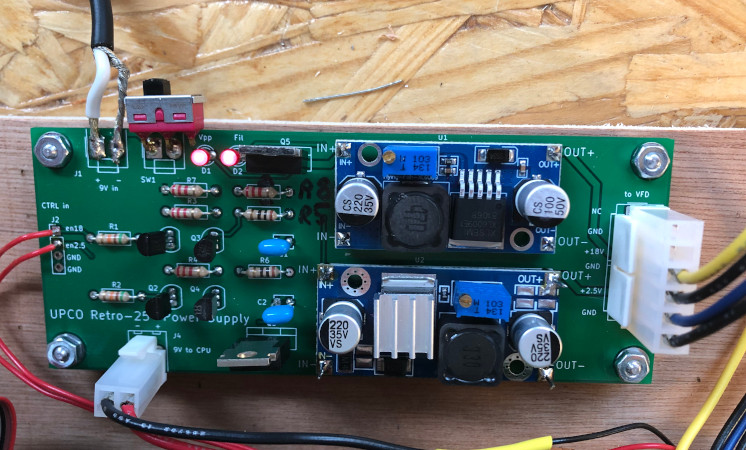
\includegraphics[width=\textwidth]{figs/power_supply2.jpg}
  \column{0.5\textwidth}
    \begin{itemize}
    \scriptsize
    \item Use Buck / Boost modules from China
    \item Simple switching logic to control from Z80
    \item Add a power switch for the whole unit
    \end{itemize}
  \end{columns}
\end{frame}

\begin{frame}
  \frametitle{Putting it All Together}


  \begin{columns}
  \column{0.5\textwidth}
    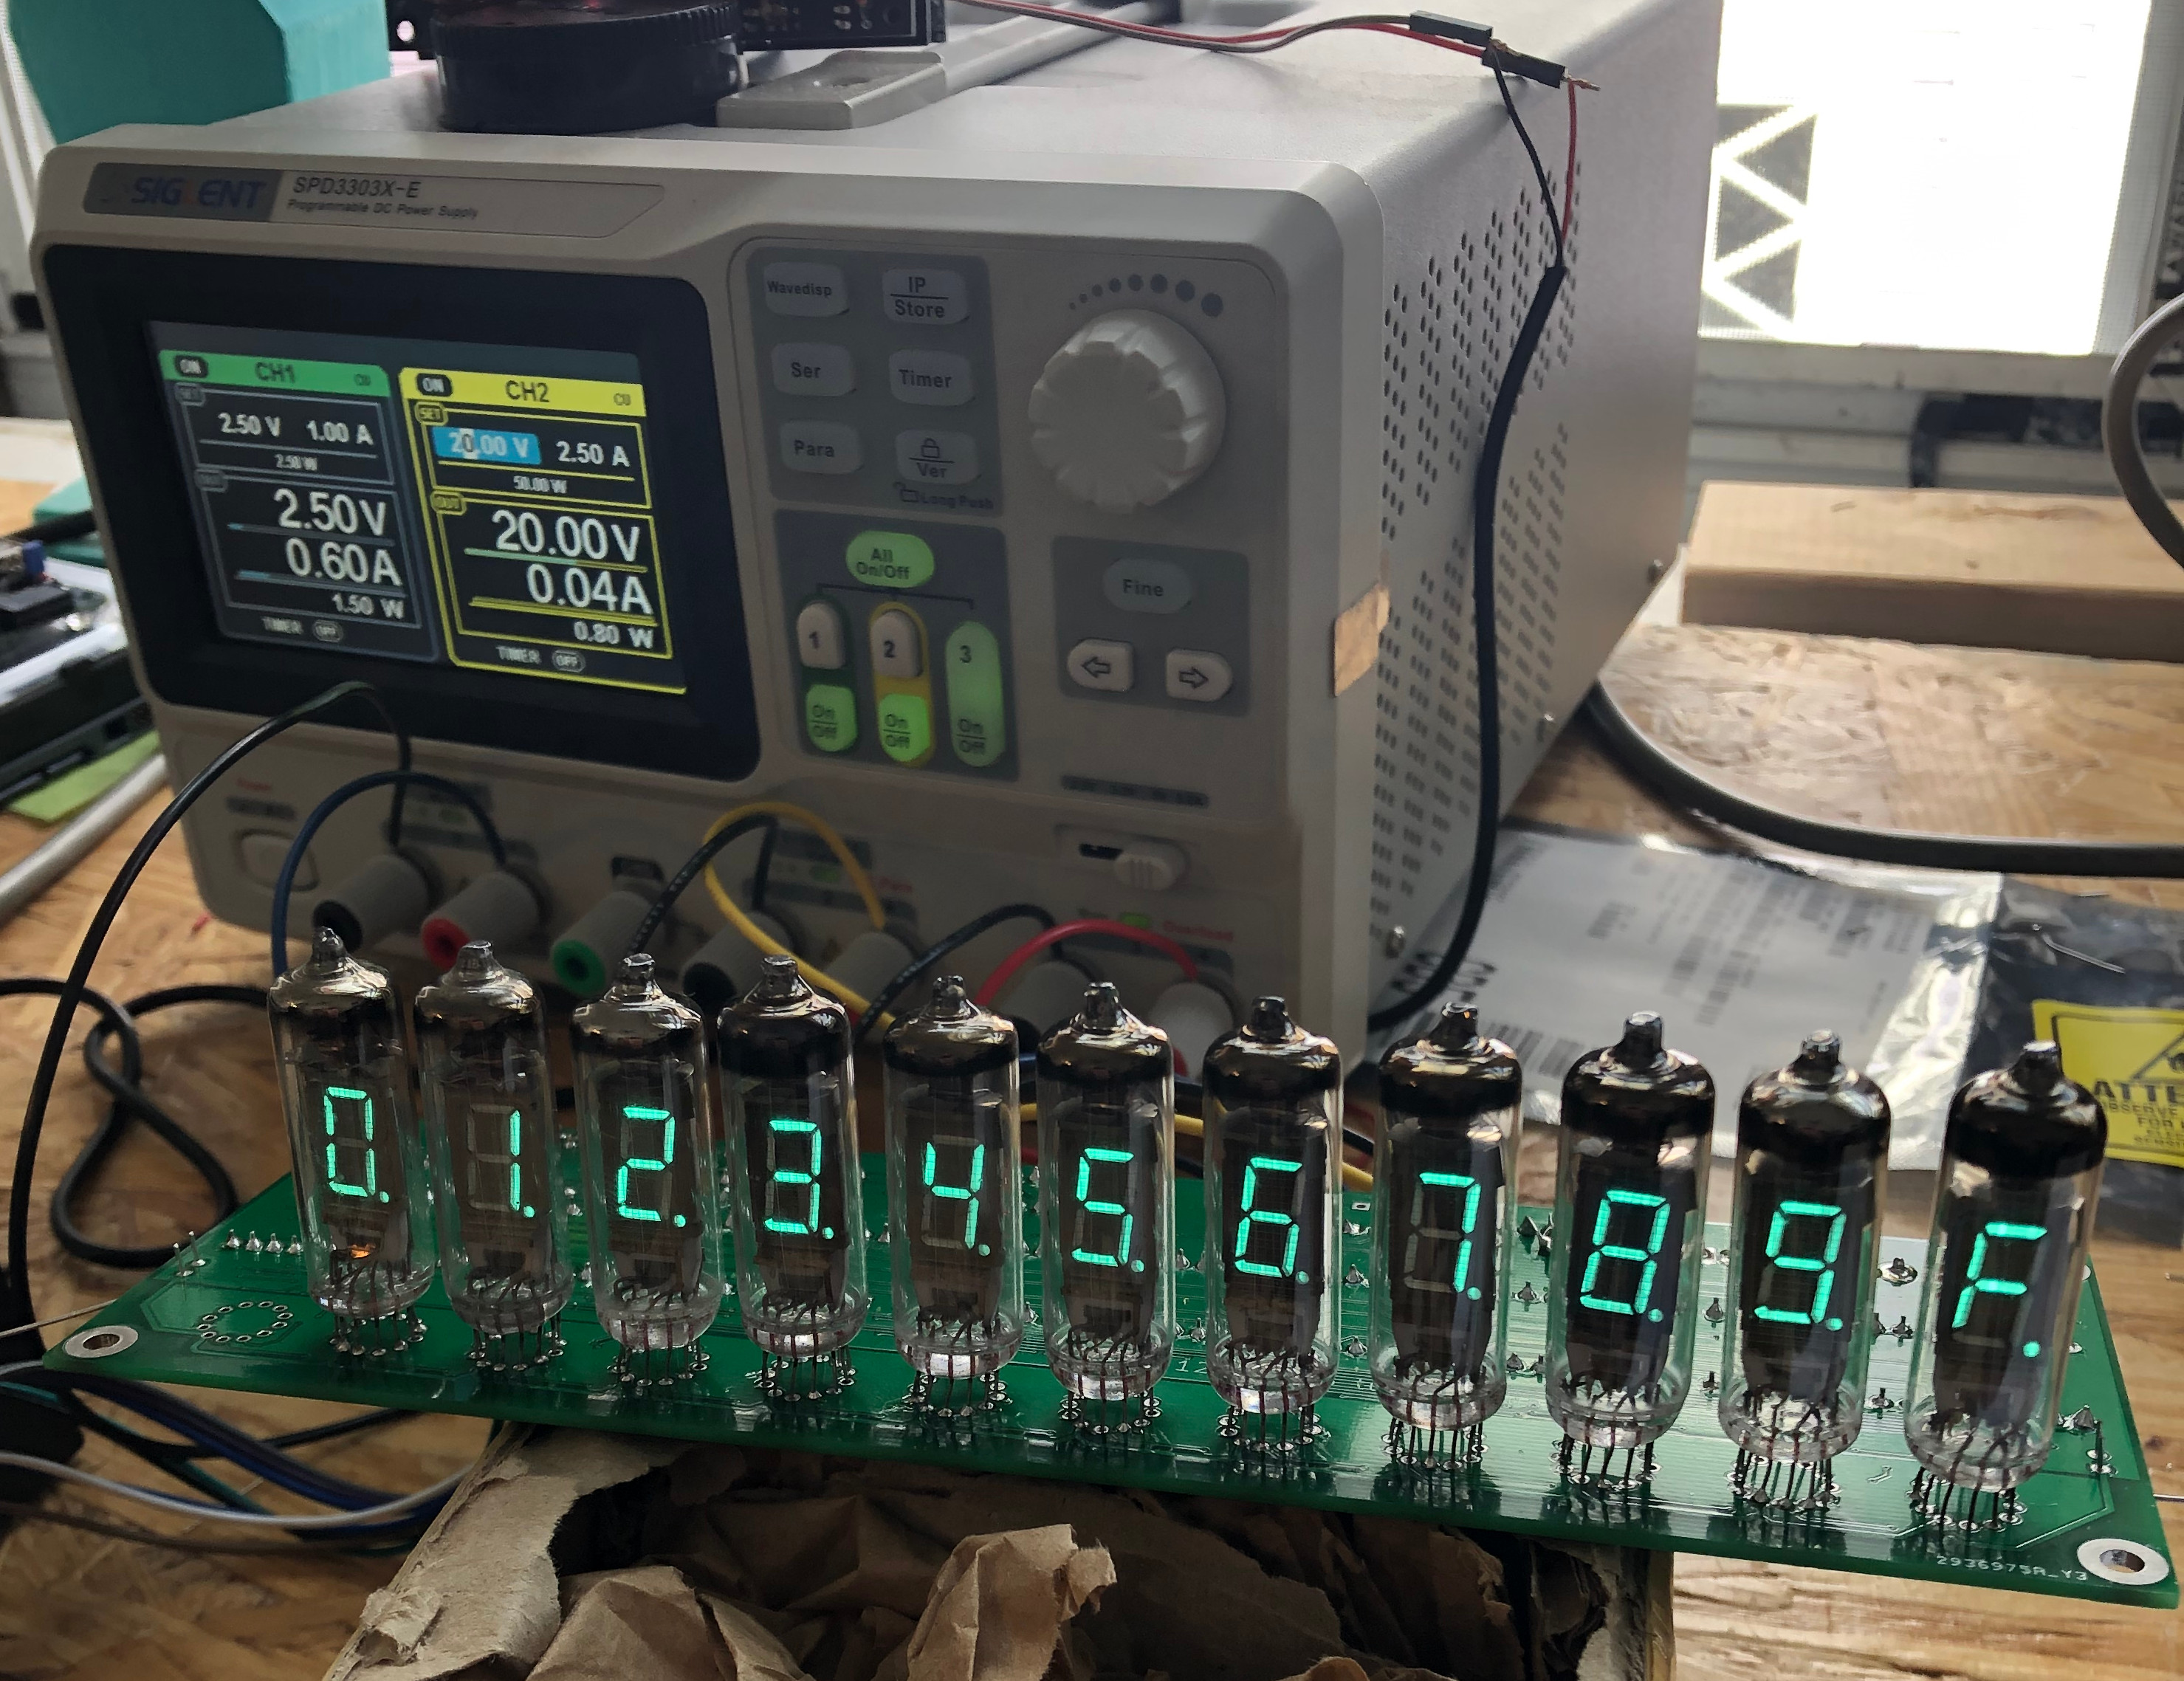
\includegraphics[width=\textwidth]{figs/display_11.jpg}
    \begin{itemize}
    \scriptsize
    \item Test the display using an Arduino
    \item Putting it all together!
    \end{itemize}
  \column{0.5\textwidth}
    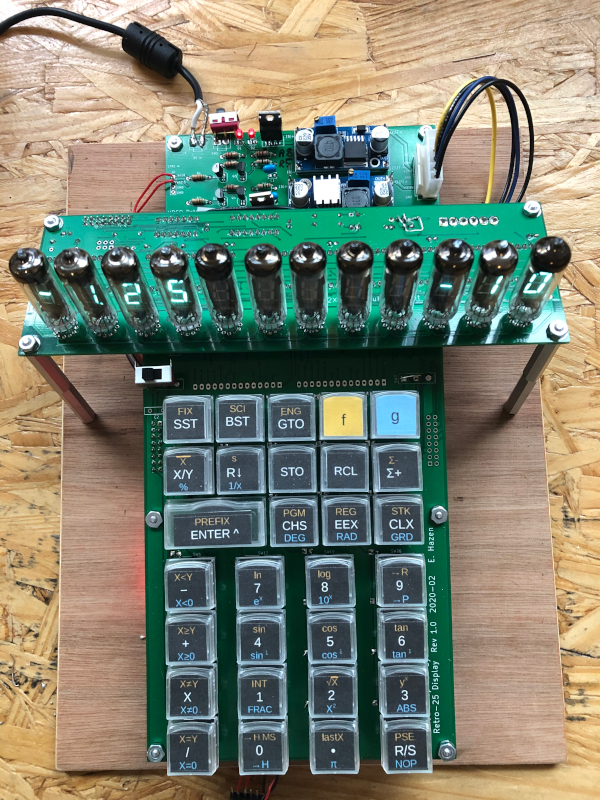
\includegraphics[width=\textwidth]{figs/top_with_ps.jpg} \\
  \end{columns}
        

\end{frame}

\end{document}
